
\chapter{Anwendungen von Algorithmen}\label{Kapitel4}
%Grundeinleitung
%Nachdem die Grundlagen der Funktionsprinzipien der Algorithmen zu Pfadplanung nun erläutert  wurden, wird nun auf mögliche Anwendungen dieser eingegangen.
\section{Anwendungen der diskreten Pfadplanung}
Die Klassifizierung des Planens im  diskreten Zustandsraum ist z.B. für das Rubik's Cube Rätsel zutreffend (siehe Abb. \ref{Abb. 5.1}), bei dem es einen endlichen Zustandsraum und einen endlichen Aktionsrahmen gibt. Der Zustandsraum ist hierbei die Summe aller möglichen Farbverteilungen, die der Würfel annehmen kann. Der Aktionsrahmen ist die Menge aller Richtungen, in die man jedes Element drehen kann. Der bestmögliche Pfad ist in diesem Fall die geringste Anzahl an Drehungen des Würfels in der richtigen Reihenfolge, um ans Ziel bzw. zum Zielzustand zu gelangen, welcher ist, dass jede Seite des Würfels nur noch Elemente einer Farbe hat \cite[~S. 20]{Lav06}.\\
\begin{figure}
	\centering
	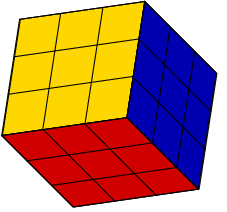
\includegraphics[width=0.4\linewidth]{images/img229}
	\caption{in Anlehnung Abb. 1.1 von \cite[~S. 5]{Lav06}: Rubik's Cube.}
	\label{Abb. 5.1}
\end{figure}%TODO Graphic bearbeiten, Pfeile einzeichnen.

Eine weitere Anwendung ist die Bewegungen eines Roboters auf einem 2D Netz. Dies geschieht in Strategie-Computerspielen, in denen eine Figur von ihrem aktuellen Standpunkt zu einem Ort gelangen muss, der ihr zugewiesen wird. Hier kommt der Pfadplanungsalgorithmus zum Einsatz \cite{cui2011based}.%TODO Quelle genauer Lesen, auf Meshes und Algorithmen eingehen, die von Bernardo und Felix schon eingeführt wurden. Evtl. Grafik übernehemen.
%s27ff
\section{Anwendungen der kontinuierlichen Pfadplanung}
Wie in Kapitel \ref{Kapitel 4.2} schon erwähnt, klassifiziert man bei den Algorithmen zur Planung mit kontinuierlichem Zustandsraum zwischen drei verschiedenen Rubriken, die unterschiedliche Anwendungsbereiche haben, auf die im Folgenden einzeln eingegangen wird.
\subsection{Anwendungen zur Planung mit allen Umgebungsinformationen vorhanden}%TODO Abgrenzungen von Anderen Unterpunkten
Eine praktische Anwendung ist das digitale Planen von Fabrik-Robotern, die ein Auto zusammensetzen sollen. In Abb. \ref{Abb. 5.2} ist das digitale Planen des automatischen An- und Abmontierens eines Scheibenwischermotors an ein Auto mittels eines CAD Modells dargestellt.
\begin{figure}
	\centering
	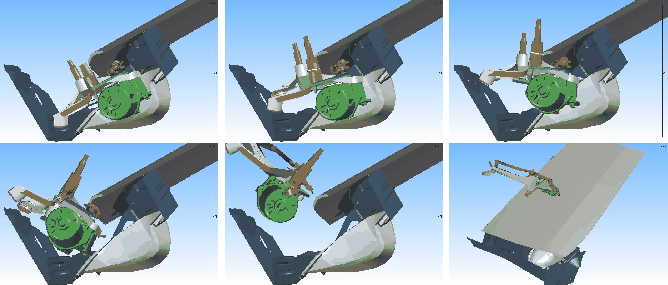
\includegraphics[width=0.7\linewidth]{images/img231}
	\caption{Abb. 1.3 von \cite[~S. 7]{Lav06}: Eine Auto-Montierungsaufgabe, die beinhaltet, dass ein Scheibenwischermotor an ein Auto angebracht oder entfernt werden soll.}
	\label{Abb. 5.2}
\end{figure}

Eine Software muss entscheiden, ob und wie der Scheibenwischermotor an- und abmontiert werden kann, oder nicht. Das früher zeit- und kostenintensive Entwickeln des Designs wird nun mit Software vereinfacht, indem CAD Modelle manipuliert werden. Auch hier hat man einen überabzählbar unendlichen Zustandsraum und alle Umgebungsinformationen sind bekannt. \cite[~S. 6 ff]{Lav06}
%part 2 QUELLE ANGEBEN
\subsection{Anwendungen zur Planung mit Unsicherheit}
Bei der Planung mit Unsicherheit (engl. planning under uncertanty), auch \textit{decision-theoretic planning} genannt, interferieren Ungewissheiten mit zwei Aspekten des Planens. Diese beiden Aspekte sind Vorhersehbarkeit und Wahrnehmung. \cite[~S. 435 ff.]{Lav06}\\
Die Vorhersehbarkeit ist in dem Sinne durch die Unsicherheiten beeinträchtigt, dass nicht bekannt ist, was passieren wird, wenn gewisse Aktionen ausgeführt werden. Die Wahrnehmung ist durch die Unsicherheiten beeinträchtigt, da der aktuelle Status, bzw. die aktuelle Position nicht bekannt ist. Denn den Status erhält man aus den Ausgangsbedingungen, den Sensoren und den Informationen über die vorangegangenen Aktionen.\\
Ein Beispiel für eine solche Anwendung ist das Autonome Fahren im Allgemeinen. %Quellen suchen
 Hier bewegt sich das Auto nicht über ein festes 2D Netz, sondern durch die unvorhersehbare Realität. Der Bordcomputer des Autos nimmt durch seine Sensoren und eventuelle Außenkameras seine Umgebung wahr und versucht durch diese und GPS-Daten, seinen Status bzw. seine aktuelle Position herauszufinden. Da sich jedoch die Umgebung stets verändert und das Verhalten der anderen Verkehrsteilnehmer nicht vorhersagbar ist, kommt die Unsicherheit ins Spiel.
Dies lässt sich auf die Navigation von allen mobilen Robotern übertragen.
Da der aktuelle Status nie gewiss sein kann, wird mit allen verfügbaren Informationen versucht, den Status so genau wie möglich zu bestimmen.
%(s.25) Part 3
\subsection{Anwendungen zur Planung mit Bewegungseinschränkungen}
Bei Anwendungen zur Planung mit Bewegungseinschränkungen (engl. planning under differential constraints) muss beachtet werden, dass der schnellste Pfad, der errechnet wird, oft durch Bewegungseinschränkungen nicht umgesetzt werden kann. In der Robotik entstehen diese Bewegungseinschränkungen häufig durch die Kinematik und Dynamik der Roboter selbst.\\
Auch hier kann gut das Auto als Beispiel herhalten. Ein Auto kann nicht seitwärts fahren. Wenn es also seitlich neben einer Parklücke steht und man mit Hilfe des Einparkassistenten das Auto einparken lassen will, wäre der kürzeste Pfad seitwärts zu fahren. Da dies nicht möglich ist, muss das bei der Pfadplanung berücksichtigt werden (siehe Abb. \ref{Abb. 5.3}).
\begin{figure}
	\centering
	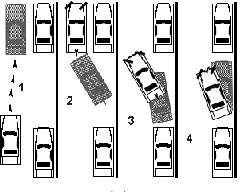
\includegraphics[width=0.5\linewidth]{images/img239}
	\caption{in Anlehnung an Abb. 1.11 von \cite[~S. 15]{Lav06}}
	\label{Abb. 5.3}
\end{figure}

%s26 Part IV